\begin{figure*}[t]
  \centering
  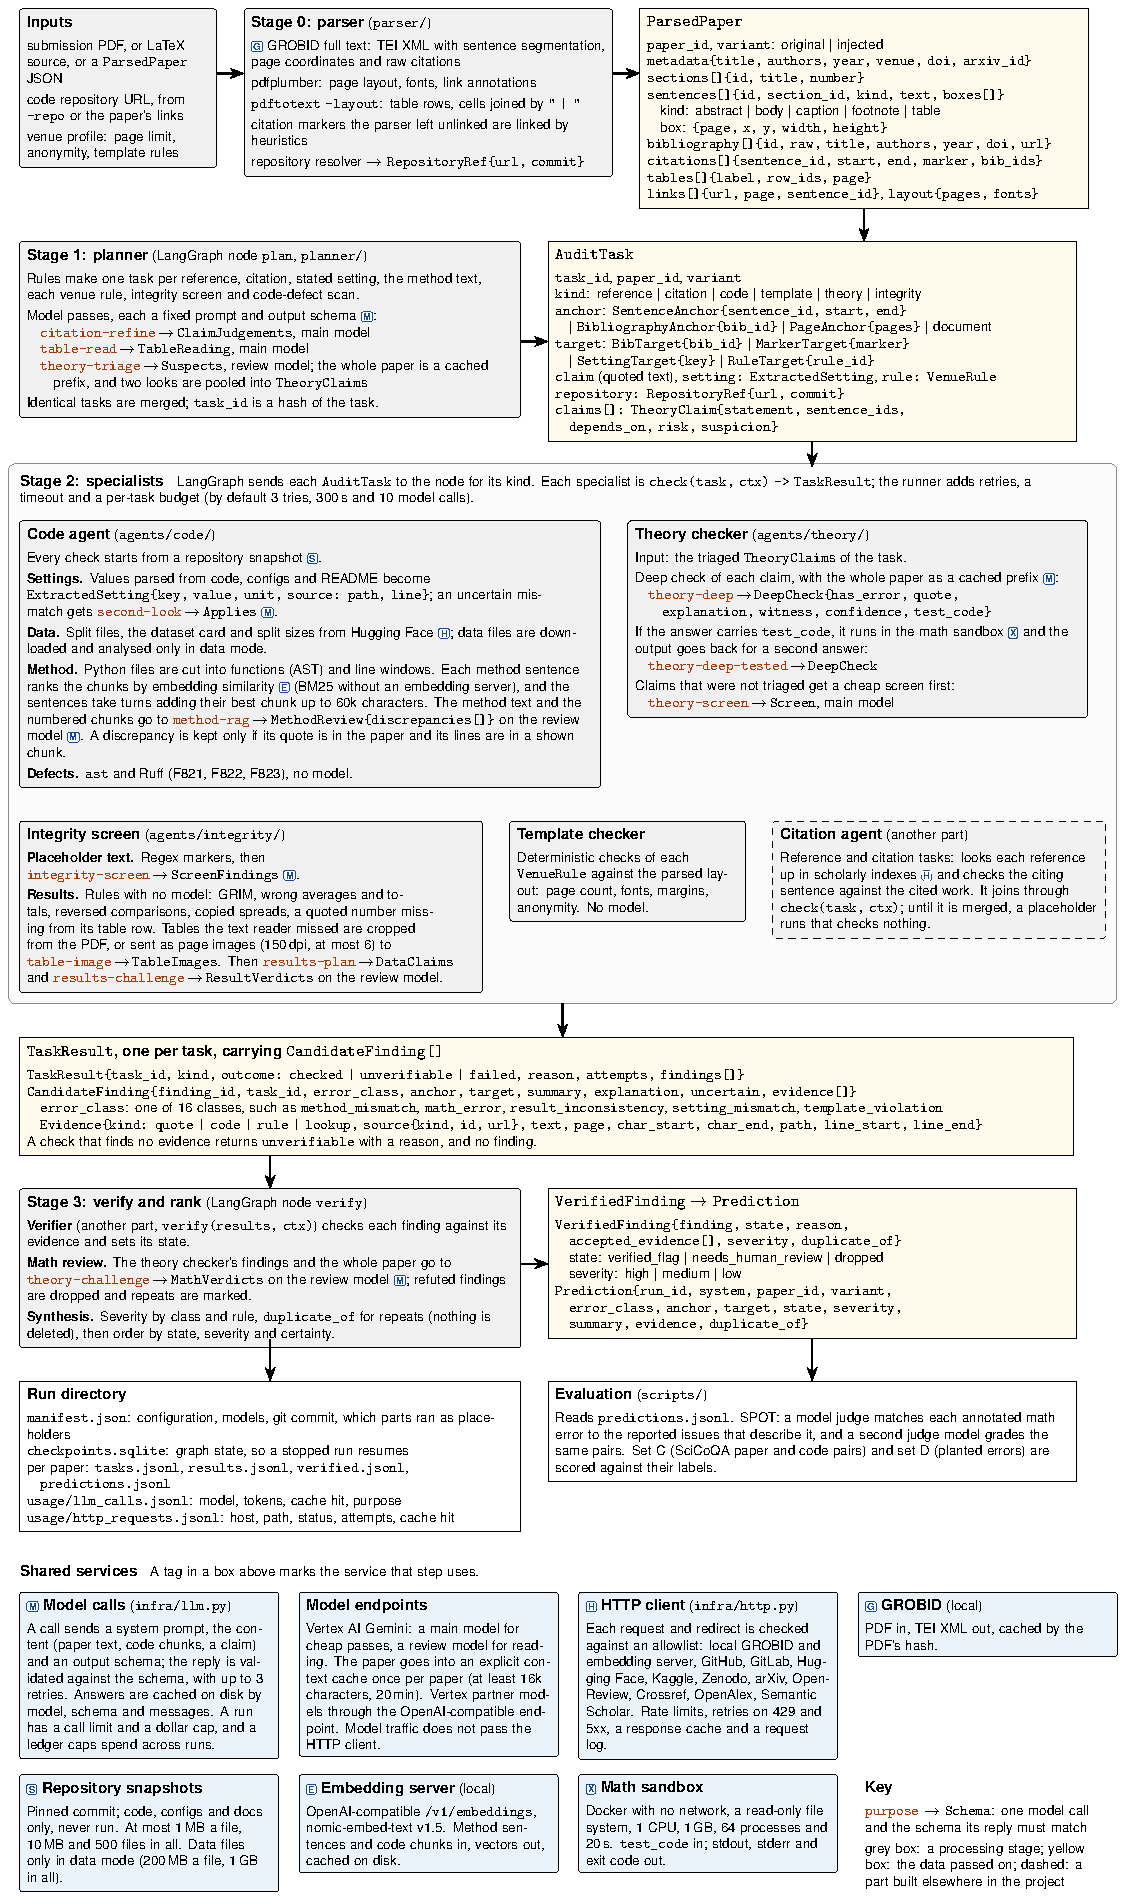
\includegraphics[width=\textwidth]{figures/architecture.pdf}
  \caption{Architecture of the auditor. Grey boxes are processing stages; yellow boxes are the
  records passed from one stage to the next, with their fields. Each model call is labelled with
  its purpose and the schema its reply must match, and a tag marks each shared service a step
  uses. All records are frozen Pydantic models that reject unknown fields. A finding names the
  sentence or code lines it is about and carries the quoted evidence. A check that finds no
  evidence reports the task as unverifiable. The citation agent and the verifier (dashed) are
  other parts of the project and plug in through the entry points shown.}
  \label{fig:architecture}
\end{figure*}
